\documentclass[12pt]{article}

\usepackage[utf8]{inputenc}
\usepackage[T2A]{fontenc}
\usepackage[english,russian]{babel}
% \usepackage[libertine]{newtxmath}
% \usepackage{xfrac,unicode-math}
% \setmathfont{Stix Math}[version=stix]
\usepackage{paratype}
\usepackage{verbatim}
\usepackage{caption}
\captionsetup[figure]{skip=1pt}
\usepackage{microtype}
\usepackage[style=numeric, sorting=none]{biblatex}
\addbibresource{refs.bib}
% \usepackage{minted}
% \usepackage{fancyhdr}
\usepackage{amssymb,amsmath,amsthm,amsfonts}
\usepackage{gensymb}
\usepackage{booktabs}
% \usepackage{mathtools}
\usepackage{geometry}
% \usepackage{titling}  
\usepackage{indentfirst}
\usepackage{graphicx}
\graphicspath{ {../vis/} }
\usepackage[table,xcdraw]{xcolor}
% \usepackage{thmtools}
\usepackage{hyperref}
% \usepackage{pdfpages}
\hypersetup{
    colorlinks=true,
    linkcolor=blue,
    filecolor=magenta,      
    urlcolor=cyan,
}
% \pgfplotsset{width=10cm, height=10cm, compat=1.16,
% tick label style={font=\normalsize},
% label style={font=\normalsize},
% legend style={font=\normalsize},} 
% \usetikzlibrary{decorations.markings}
% \usetikzlibrary{arrows.meta}
% \usepgfplotslibrary{fillbetween}
% \pgfplotsset{mast1/.style={
%         width=6cm, height=6cm,
%         % axis on top,
%         axis equal,
%         axis lines = center,
%         tick style={draw=none},
%         legend pos = south east,
%         enlargelimits=false,
%         axis background/.style={fill=backcolor},
%         }}

\usepackage{tocloft}
\renewcommand{\cftsecleader}{\cftdotfill{\cftdotsep}}
% \usepackage{fancyhdr}
\geometry{a4paper, textwidth=16cm, textheight=24cm}
\setcounter{secnumdepth}{0}
% \newtheorem{remark}{Замечание}
\usepackage[italic]{mathastext}

\title{Отчет по заданию №1:\break Метрические алгоритмы классификации}
\author{Васильев Руслан \and{ВМК МГУ, 317 группа}}

\begin{document}

\maketitle
\tableofcontents

\section{Введение}
В рамках задания требовалось реализовать метод k-ближайших соседей, инструменты для кросс-валидации и функции для вычисления попарных расстояний. В данном отчете описывается ход и результаты экспериментов, произведенных с помощью написанных программ на датасете MNIST. Далее, согласно заданию, предполагается следующее разбиение: первые 60~000 объектов (обучающая выборка) и последние 10~000 (тестовая выборка).

\section{Какой алгоритм работает быстрее? (№1)}

В первом эксперименте сравнивается время работы доступных алгоритмов реализованного классификатора. Для этого производится поиск 5 ближайших соседей для каждого объекта тестовой выборки, по евклидовой метрике. Размер блока для вычислений~--- 1000 объектов, причем этот параметр используется только для методов, которые строят в памяти матрицу попарных расстояний (\verb|my_own| и \verb|brute|). 

\begin{figure}[!h]
    % \centering
    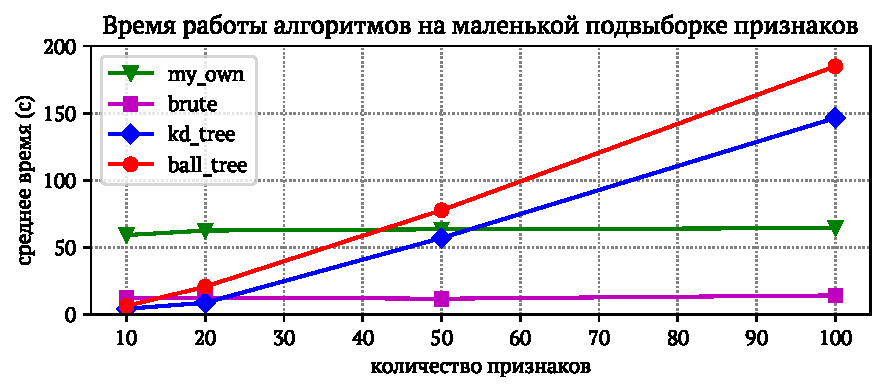
\includegraphics{n1_1}
    \caption{}
    \label{fig:time1}
\end{figure}


На \autoref{fig:time1} видно, что деревья имеют преимущество только в случае малого числа признаков~--- в данном случае 10 для обоих алгоритмов, а также для 20 в случае \verb|kd_tree|. Сравнивая сами деревья, видим, что Ball tree уступает KD tree. На время работы переборных реализаций количество признаков почти не влияет. Посмотрим, что произойдет, если учитывать еще больше доступных признаков.

\begin{figure}[h]
    % \centering
    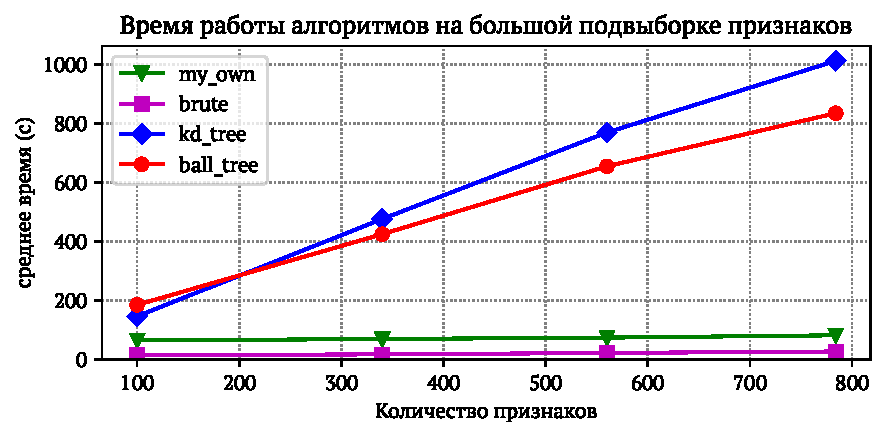
\includegraphics{n1_2}
    \caption{}
    \label{fig:time2}
\end{figure}

\hyperref[fig:time2]{Рис. 2} показывает, время работы алгоритмов, основанных на деревьях, сильно возрастает с ростом числа признаков. Это неочевидный результат, поскольку в теории время поиска ближайшего соседа имеет (в среднем) время работы зависит логарифмически от размера обучающей выборки, в отличие от полного перебора, где зависимость уже линейная. Такую асимптотику нужно интерпретировать с осторожностью~--- в ней не учитывается размерность пространства признаков. Для действительно логарифмической сложности поиска в дереве необходимо потребовать его сбалансированность и равномерное распределение точек в пространстве, что существенно зависит от размерности признакового пространства в случае \verb|kd_tree| и \verb|ball_tree|. Причина невыполнения этих свойств~--- проклятие размерности: 60~000 даже равномерно распределенных объектов недостаточно для равномерного покрытия по нескольким сотням признаков.

Наконец, время работы \verb|brute| и \verb|my_own| с ростом признаков по-прежнему меняется незначительно, что связано с векторизацией вычислений попарных расстояний. Далее будем использовать только эти алгоритмы, поскольку, как мы показали выше, деревья в данной задаче работают неэффективно.

\section{Какую использовать метрику и нужны ли веса? (№2, №3)}

Целью данного эксперимента, кроме ответа на поставленные вопросы, является измерение времени кросс-валидации, а также подбор оптимального значения $k$~--- числа ближайших соседей.

Разумным функционалом качества для данной задачи является точность~--- доля верных предсказаний классификатора. Валидация происходит на 3-фолдах: соседи ищутся в пределах от 1 до 10, в качестве метрик рассматриваются евклидова и косинусная.

В эксперименте использовались алгоритмы и \verb|my_own|, и \verb|brute|, но, как и следовало ожидать, при одинаковых гиперпараметрах они дают одинаковые предсказания~--- поэтому результаты в измерении точности оказались равными.

\begin{figure}[h]
    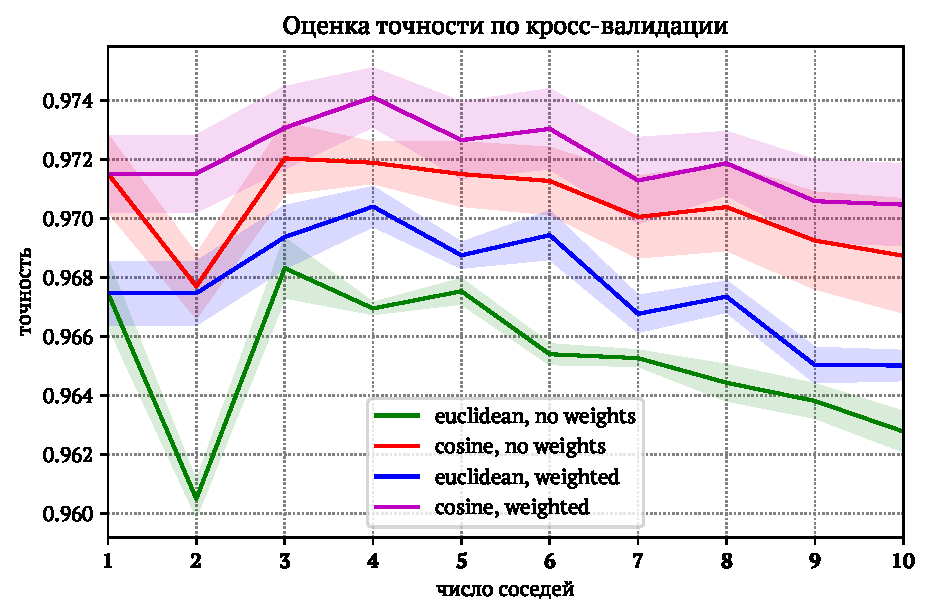
\includegraphics{n23_acc}
    \caption{Полупрозрачным обозначено стандартное отклонение}
    \label{fig:cv_acc}
\end{figure}

Кросс-валидация показывает, что \emph{косинусная метрика дает более точные предсказания, чем евклидова, и использование весов также улучшает качество классификации}. Отметим, что весовые коэффициенты в метрических алгоритмах можно использовать по-разному: они могут зависеть от номера ближайшего соседа, от расстояния до него и от выбора самой функции. В данной реализации голос одного сосдеда полагается равным $\frac{1}{d+10^{-5}}$, где $d$~--- расстояние между объектом и рассматриваемым соседом.

Также~\autoref{fig:cv_acc} показывает, что оптимально использование метода 4-х ближайших соседей. Четность не мешает как раз из-за весов.

Итак, лучшая средняя точность по кросс-валидации составляет \textbf{97.41\%} (в тексте отчета будет использоваться выражение точности процентах), которая получается с использованием взвешенного метода $k=4$ ближайших соседей и косинусной метрикой.

Также по заданию требовалось измерить время поиска соседей в процессе кросс-валидации. Эффективная реализацию заключается в том, чтобы сразу посчитать расстояния до максимального исследуемого числа соседей, а затем последовательно <<отбрасывать лишних>>. Соответствующий результат приведен на \autoref{fig:cv_times}.

\begin{figure}[h]
    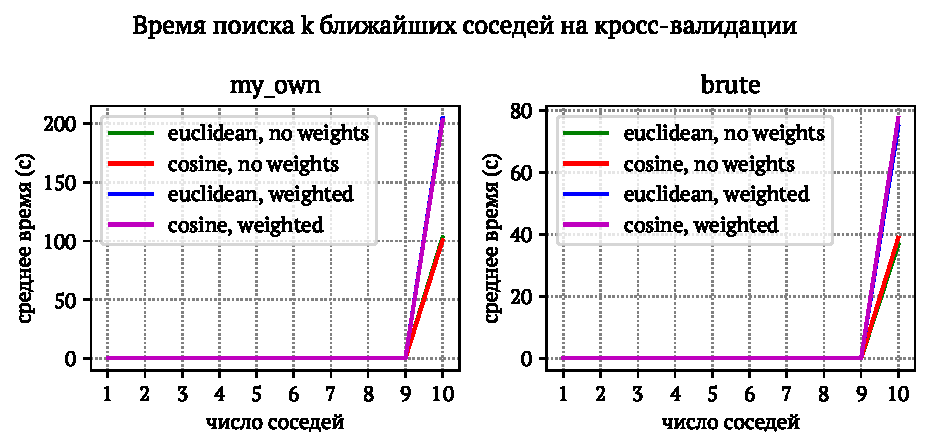
\includegraphics{n23_cv_times}
    \caption{}
    \label{fig:cv_times}
\end{figure}

Как и следовало ожидать, единственное трудоемкой операцией является поиск 10 соседей, дальнейшие же вычисления не времязатратны. Наложение кривых связано с одинаковой сложностью вычислений матриц попарных расстояний для евклидовой и косинусной метрик. Подобно достаточно известной оптимизации для евклидовой метрики \cite{eumatrix}, следующее очевидное преобразование позволило быстрее посчитать и матрицу попарных расстояний для косинуса:
\begin{equation}
    \rho_{\scriptscriptstyle{cos}}(\mathbf{x},\mathbf{y}) = 1-\frac{\langle\mathbf{x}, \mathbf{y}\rangle}
    {\Vert{\mathbf{x}}\Vert \cdot \Vert{\mathbf{y}}\Vert} = 
    1-\left\langle
        \frac{\mathbf{x}}{\Vert{\mathbf{x}}\Vert},
        \frac{\mathbf{y}}{\Vert{\mathbf{y}}\Vert}
    \right\rangle
\end{equation}

То есть достаточно сначала произвести нормировку признакового описания объектов, а затем умножить матрицы. Такой подход, использованный в реализации библиотеки scikit-learn \cite{sklearn_api}, использует только $(l_1 + l_2) \cdot d$ делений, в то время как нормировка после матричного перемножения потребует $O(l_1\cdot l_2)$ делений, где $d$~--- размерность признакового пространства, а $l_1$ и $l_2$~--- число объектов (в нашем случае строк) в соответственно первой и второй матрице.

\section{Качественная ли получилась модель? (№4)}

В данном эксперименте мы обучим модель с полученными гиперпараметрами на всей обучающей выборки и проанализируем предсказания на тестовой.

Итак, качество на тесте~--- \textbf{97.52\%}, что превосходит среднюю точность той же модели на кросс-валидации (97.41\%). Различие не столь значительное, хотя обычно точность на тесте получается ниже. На самом деле точность на кросс-валидации  зависит от способы разбиения на фолды: можно было бы делать равные пропорции классов, случайно перемешивать, брать другое число подвыборок. В нашей реализации используется стандартное последовательное разбиение на фолды, поскольку датасет MNIST уже перемешан. 

Согласно рейтингу \cite{topmnist}, лучшее качество в известных работах~---~\textbf{99.84\%}~\cite{byerly2020branching}, \mbox{результат} 2020-го года. Авторы используют сверточные нейронные сети, предсказания которых улучшются с помощью аугментации и специальных методов ансамблирования.

Вернемся к нашей модели.

\begin{figure}[h]
    \centering
    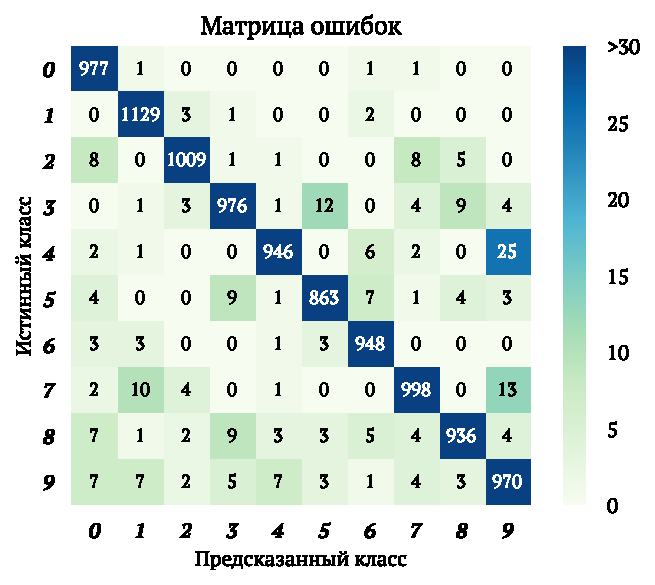
\includegraphics{4_conf}
    \caption{}
    \label{fig:conf_bl}
\end{figure}

\begin{centering}
    \begin{table}[h]
        \begin{tabular}{@{}ccccccccccc@{}}
        \toprule
        \textbf{\begin{tabular}[c]{@{}c@{}}истинный\\ класс\end{tabular}}                                                        & 0                                    & 1    & 2    & 3     & 4     & 5     & 6    & 7     & 8                                    & 9                                     \\ \midrule
        \textbf{\begin{tabular}[c]{@{}c@{}}число\\ ошибок\end{tabular}}       & {\color[HTML]{32CB00} \textbf{3}}    & 6    & 23   & 34    & 36    & 29    & 10   & 30    & 38                                   & {\color[HTML]{FE0000} \textbf{39}}    \\
        \textbf{\begin{tabular}[c]{@{}c@{}}\% среди\\ ошибок\end{tabular}}     & {\color[HTML]{32CB00} \textbf{1.21}} & 2.42 & 9.27 & 13.71 & 14.52 & 11.69 & 4.03 & 12.10 & 15.32                                & {\color[HTML]{FE0000} \textbf{15.73}} \\
        \textbf{\begin{tabular}[c]{@{}c@{}}\% ошибок\\ в классе\end{tabular}} & {\color[HTML]{32CB00} \textbf{0.31}} & 0.53 & 2.23 & 3.37  & 3.67  & 3.25  & 1.04 & 2.92  & {\color[HTML]{FE0000} \textbf{3.90}} & 3.87                                  \\ \bottomrule
        \end{tabular}
        \caption{Статистики ошибок полученной модели}
        \label{tab:res4}
        \end{table}
\end{centering}

Построенная матрица ошибок (\autoref{fig:conf_bl}), а также \autoref{tab:res4} позволяют сделать следующие наблюдения:
\begin{itemize}
    \item Лучше всего модель классифицирует \textit{\textbf{0}} и \textit{\textbf{1}}. Это связано прежде всего с <<простотой>> данных символов.
    \item Самый частый вид ошибки~--- подмена \textit{\textbf{4}} (истина) на \textit{\textbf{9}} (предсказание), а также \textit{\textbf{7}} на \textit{\textbf{9}}. Обратные подстановки происходят сравнительно реже. И в основном ошибки не симметричны.
    \item Тем не менее алгоритм нередко путает \textbf{\textit{3}} и \textbf{\textit{5}} друг с другом.
    \item Чаще всего алгоритм ошибается на \textit{\textbf{8}} и \textit{\textbf{9}}. Причем \textit{\textbf{9}} еще и самая частая подмена.
\end{itemize}

Среди ошибочных классификаций выделяются разные группы с общими свойствами. Так, например, на \autoref{fig:4_rot} видно, что некоторые цифры имеют выраженный поворот покруг центра.


Цифры на некоторых изображениях (\autoref{fig:4_similar}) могут двояко классифицироваться даже человеком.

\begin{figure}[h]
    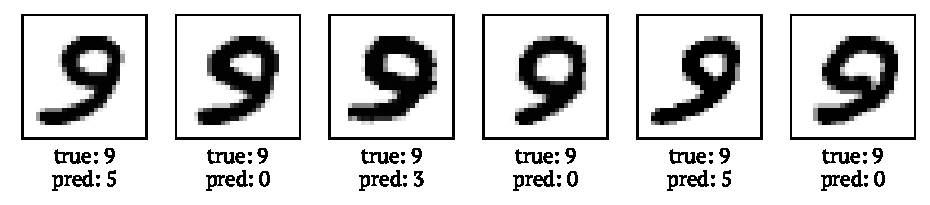
\includegraphics{4_nines_rot.pdf}

    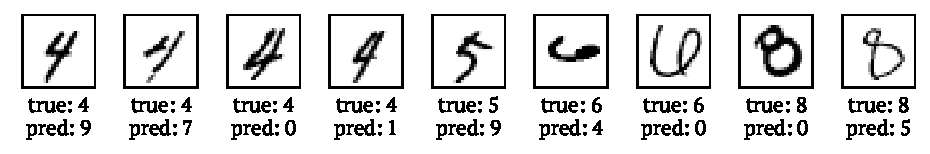
\includegraphics{4_rot.pdf}
    \caption{<<Повернутые>> цифры}
    \label{fig:4_rot}
\end{figure}
\begin{figure}[h]
    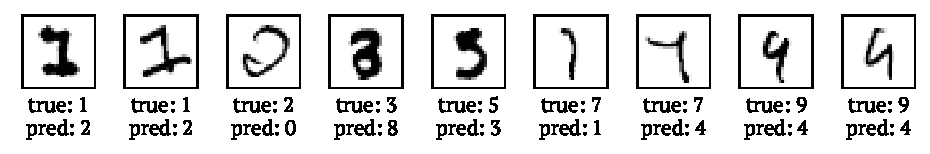
\includegraphics{4_similar.pdf}
    \caption{Цифры, допускающие несколько классификаций}
    \label{fig:4_similar}
% \end{figure}
% \begin{figure}[h]
    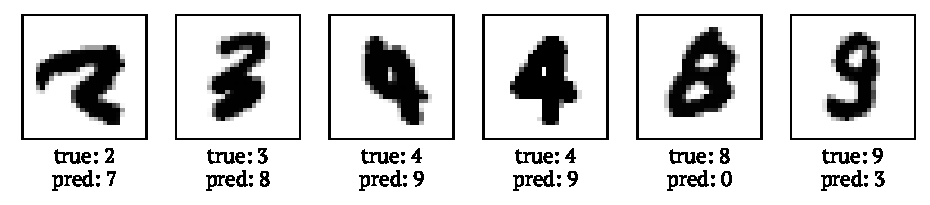
\includegraphics{4_bold.pdf}
    \caption{Слишком жирный шрифт}
    \label{fig:4_bold}
% \end{figure}
% \begin{figure}[h]
    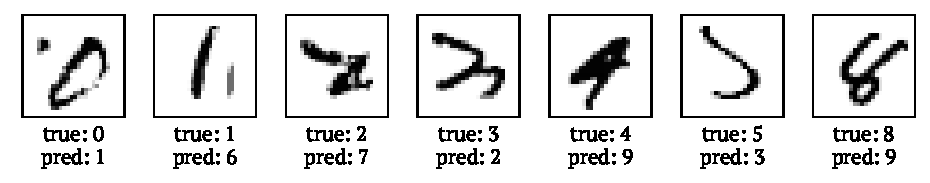
\includegraphics{4_peculiar.pdf}
    \caption{Трудно классифицируемые цифры}
    \label{fig:4_peculiar}
\end{figure}

Другие (\autoref{fig:4_bold}) цифры просто слишком жирно написаны, и их бы следовало несколько размыть.


Наконец, в датасете есть совсем необычно (\autoref{fig:4_peculiar}) написанные цифры.

\section{Аугментация данных (№5)}

В данном эксперименте требовалось увеличить количество объектов обучающей выборки посредством поворотов, смещений и применения фильтра Гаусса. Функции, связанные с обработкой изображений и аугментацией, реализованы в модуле \verb|augmentation.py|. Из-за удобного API в качестве библиотеки для работы с изображениями используется модуль \verb|scipy.ndimage|. Но его функции принимают на вход единственное изображение, поэтому были написаны распараллеленные (с помощью \verb|joblib| функции трансформации выборки.

С изменением числа объектов в обучающей выборки может измениться оптимальное количество ближайших соседей. Поэтому в процессе кросс-валидации исследуются не только разные параметры трансформаций, но и зависимость от гиперпараметра $k$.

Преобразования выборки организованы следующим образом: повороты на $\pm5\degree$, $\pm10\degree$, $\pm15\degree$; сдвиги на $\pm1$, $\pm2$, $\pm3$, пикселя по горизонтали и аналогично по вертикали; размытие с помощью фильтра Гаусса с параметром $\sigma$, равным 0.5, 1 или 1.5. Например, в случае сдвигов одна размноженная обучающая выборка может состоять из втрое большего числа объектов~--- сдвиги берутся в паре по одной оси.

Результаты кросс-валидации приведены на \autoref{fig:5_cv}. Для большей ясности дополнительно пунктиром приводится график лучшей неразмноженной модели из предыдущих экспериментов, гиперпараметры которой используются в моделях с аугментацией. Полупрозрачным цветом по-прежнему обозначается стандартное отклонение.

\begin{figure}[!h]
    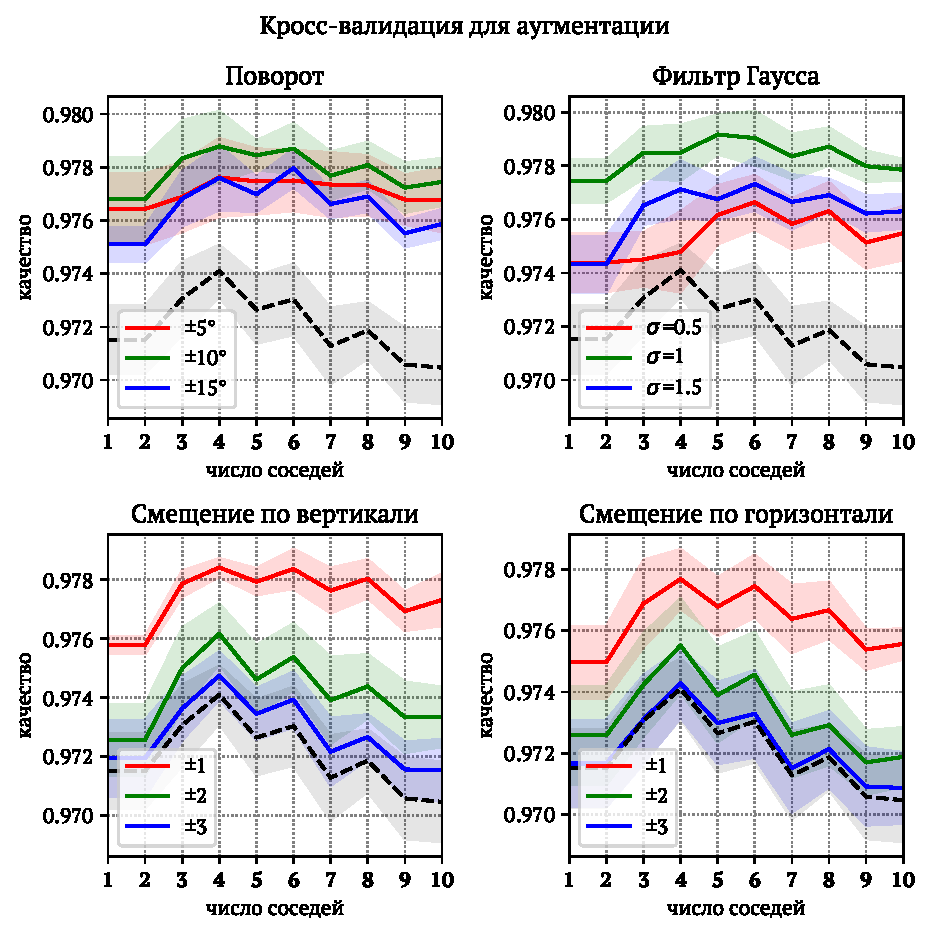
\includegraphics{5_cv}
    \caption{}
    \label{fig:5_cv}
    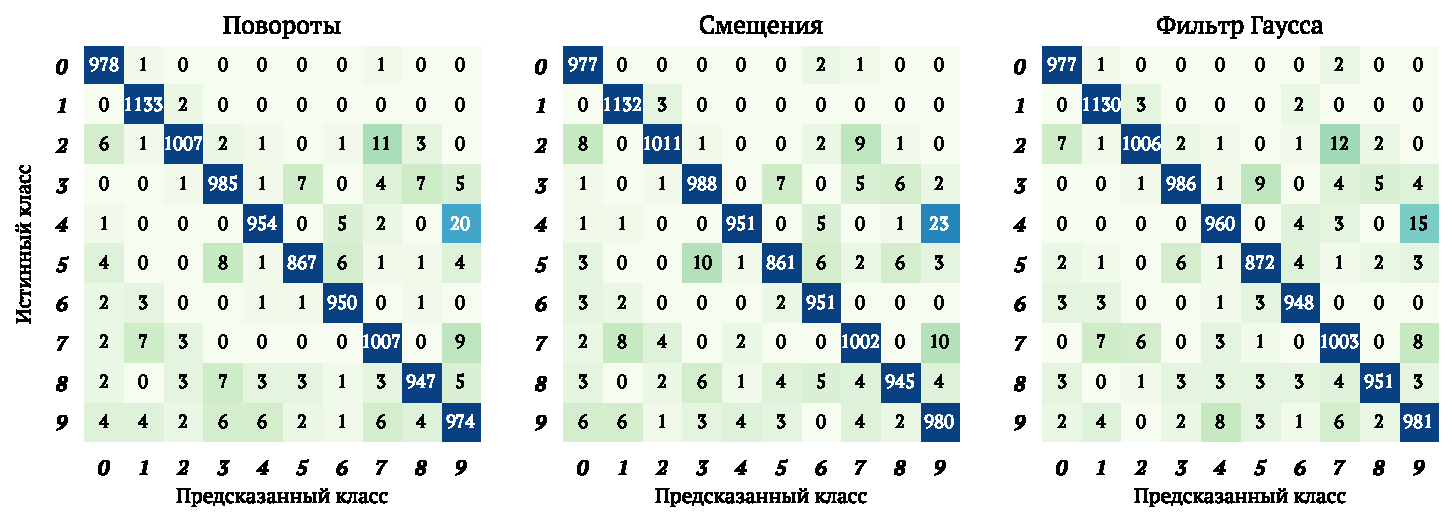
\includegraphics[width=\textwidth]{5_conf}
    \caption{}
    \label{fig:5_conf}
\end{figure}

Теперь мы можем определить лучшие параметры трансформаций: поворот на $\pm10\degree$, смещение на $\pm1$ пиксель и $\sigma=1$ в фильтре Гаусса. Далее мы объеденим сдвиги по разным осям.

Кросс-валидация показывает, что несмотря на размножение объектов обучающей выборки, параметр $k=4$ остается достаточно оптимальным (хотя при некоторых преобразованиях лучшим оказываются 5 или 6).

Изменение точности на тестовой выборки при каждом типе преобразований (с лучшими параметрами) и их комбинациями показано в \autoref{tab:final_res}. Лучшее качество достигается при сочетании сдвигов и фильтра Гаусса~--- \textbf{98.36\%}. Тем не менее использование поворотов дало наиболее интерпретируемый результат~--- чуть больше половины ошибок, показанных на \autoref{fig:4_rot}, были исправлены именно с помощью поворотов объектов обучающей выборки. Размытие фильтра Гаусса исправило часть (3 из 6) ошибок, допущенных на чересчур жирных цифрах (\autoref{fig:4_bold}). Смещения, исправили ошибки на недостаточно центрированных объектах.

Что касается изменения матрицы ошибок \autoref{fig:5_conf}, то интересно что не все подмены были исправлены трансформациями: например, \textit{\textbf{2}} стала только чаще называться \textit{\textbf{7}} в любой форме аугментации. Фильтр Гаусса уменьшил число самой распространенной ошибки~--- подмены \textit{\textbf{4}} на \textit{\textbf{9}}, а также \textit{\textbf{7}} на \textit{\textbf{9}}. Повороты достаточно равномерно уменьшили число ложных предсказаний \textit{\textbf{0}}. А \textit{\textbf{2}} и \textit{\textbf{4}} лучше всего предсказываются при смещениях.

Таким образом, с помощью аугментации можно исправлять ошибки алгоритма, причем различиные преобразования влияют на качественно разные ошибки.

% \newpage
\section{Аугментация наоборот? (№6)}

Если в предыдущем эксперименте мы размножали объекты обучающей выборки, то в заключительном мы размножим объекты теста. Такой метод часто называют test time augmentation (TTA) \cite{tta}. В нашем случае идея заключается в поиске расстояний при различных преобразованиях тестовой выборки. Далее с этими расстояниями можно поступать по-разному. Первым вариантом было усреднение, но в ходе кросс-валидации оказалось, что такой подход ухудшает модель. Более качественный результат дало не усреднение, а выбор \emph{наименьшего} из полученных расстояний~--- такая эвристика согласуется с идеей метода $k$ ближайших соседей.

Выбор параметров трансформаций производился по той же схеме, что и при аугментации. Результаты можно видеть на \autoref{fig:6_cv}. Лучшие варианты для поворотов и смещений остались без изменений, а вот фильтр Гаусса во всех случаях ухудшал качество. Для единообразия возьмем $\sigma=1$.

Как и в случае аугментации, повороты снова помогают исправить ошибки на <<повернутых>> изображениях \autoref{fig:4_rot}, а фильтр Гаусса в TTA справился с задачей \autoref{fig:4_bold} хуже.

Лучшая точность~--- \textbf{98.35\%} достигается в случае комбинации поворотов и сдвигов.

\begin{figure}[!h]
    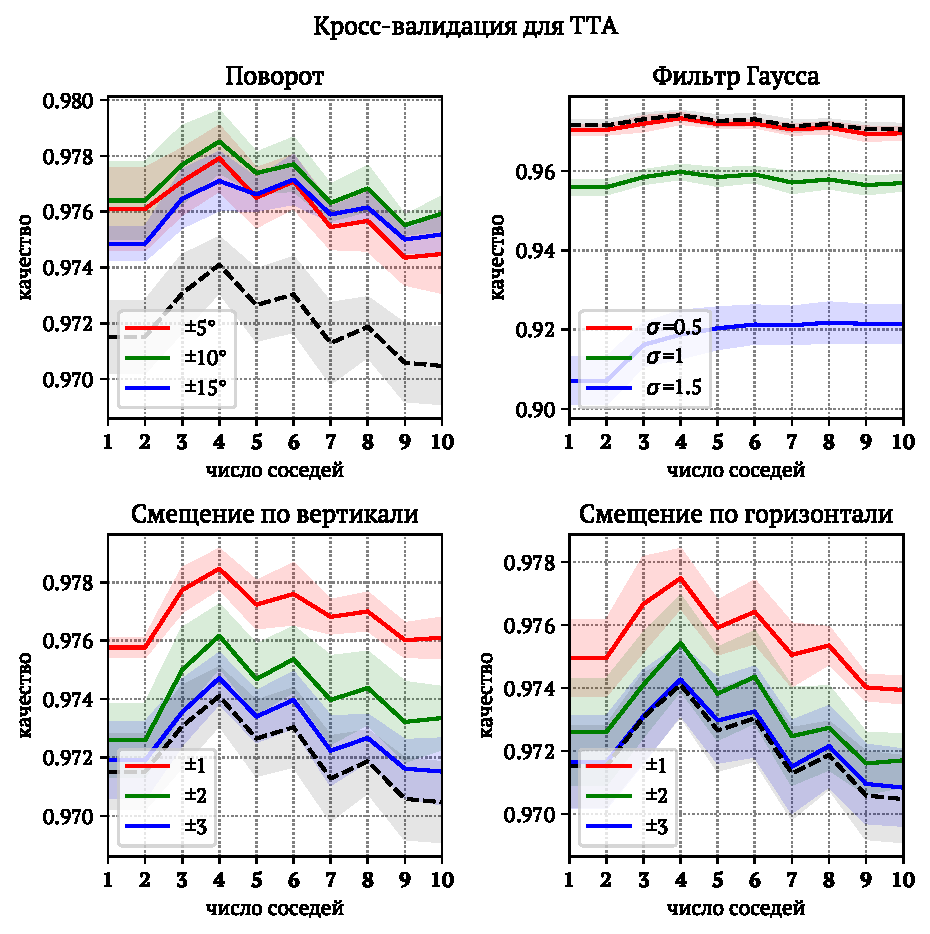
\includegraphics{6_cv}
    \caption{}
    \label{fig:6_cv}
    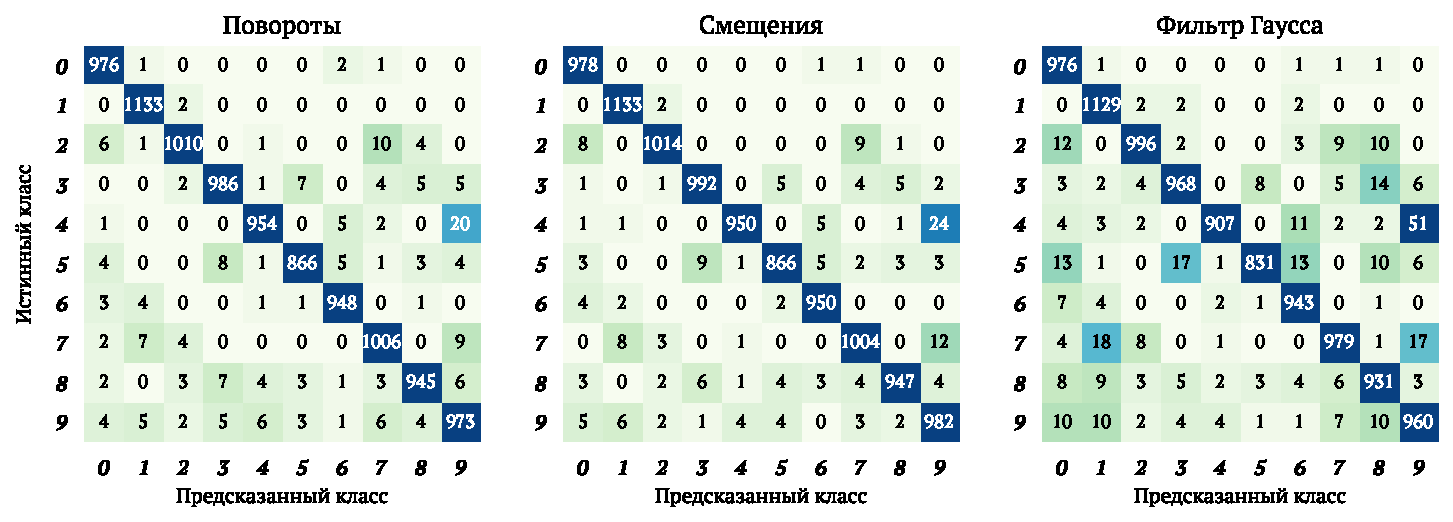
\includegraphics[width=\textwidth]{6_conf}
    \caption{}
    \label{fig:6_conf}
\end{figure}

 На матрице ошибок \autoref{fig:6_conf} особенно хорошо видно, как фильтр Гаусса ухудшает модель в случае TTA. Причина может быть в том, что его применение призвано уменьшить шум, что в случае аугментации действительно полезно. <<Стирая>> же часть информации с классифицируемого объекта, мы теряем часть информации и делаем его еще более похожим на другие классы. В то же время, и смещения, и повороты действуют в TTA схожим с аугментацией образом. Однако аугментация более эффективно справляется со сдвигами, в то время как TTA~--- с поворотами. Финальное сравнение точности двух методов на тестовой выборке при различных комбинациях преобразований приведено на \autoref{tab:final_res}.

\begin{center}
\begin{table}[h]
    \begin{tabular}{@{}cccccccc@{}}
        \toprule
            & \begin{tabular}[c]{@{}c@{}}повороты\\ $\pm10\degree$\end{tabular} & \begin{tabular}[c]{@{}c@{}}сдвиги\\ $(\pm1,\pm1)$\end{tabular} & \begin{tabular}[c]{@{}c@{}}фильтр\\ Гаусса\\ $\sigma=1$\end{tabular} & \begin{tabular}[c]{@{}c@{}}повороты\\ +\\ сдвиги\end{tabular} & \begin{tabular}[c]{@{}c@{}}повороты\\ +\\ Гаусс\end{tabular} & \begin{tabular}[c]{@{}c@{}}сдвиги\\ +\\ Гаусс\end{tabular} & \begin{tabular}[c]{@{}c@{}}повороты,\\ сдвиги,\\ Гаусс\end{tabular} \\ \midrule
        AUG & 98.02                                                             & 97.98                                                          & 98.14                                                                & 98.30                                                         & 98.33                                                        & \textbf{98.36}                                             & 98.30                                                               \\
        TTA & 97.97                                                             & 98.16                                                          & 96.20                                                                & \textbf{98.35}                                                & 96.53                                                        & 96.52                                                      & 96.52                                                               \\ \bottomrule
        \end{tabular}
    \caption{Сопоставление подходов №5 и №6. Точность модели в процентах. Для сравнения, точность, полученная в эксперименте №5 составила \textbf{97.52\%}.}
    \label{tab:final_res}
\end{table}
\end{center}

\section{Заключение}
Таким образом, на примере классификации изображений мы провели целый ряд экспериментов с $kNN$. В нашей задаче лучшим образом себя проявила косинусная метрика, которая применяется не столь часто. Были сопоставлены два различных метода размножения выборок, и хотя оба имели свои преимущества, лучший результат показала аугментация, основанная на преобразованиях смещения и фильтра Гаусса. Итоговое качество~--- \textbf{98.36\%}.


\section{Параллелизм}
В качестве небольшого дополнения отметим роль параллельных вычислений в метрических алгоритмах. Действительно, поиск ближайших соседей может проходить независимо, поэтому нет причин не использовать всю вычислительную способность компьютера. Единственное препятствие~--- рамер оперативной памяти, но библиотека \verb|joblib|, использованная в реализации модулей, позволяет также использовать отображения фрагментов диска. Таким образом, получается эффективно работать с отдельными сегментами матрицы попарных расстояний, не храня ее полностью в оперативной памяти. Параллельная реализация поиска ближайших соседей написана в методе \verb|KNNClassifier._fkn_parall|. Другое полезное использование параллельных вычислений~--- трансформации изображений (\verb|augmentation.py|).

\selectlanguage{english}
\printbibliography
\end{document}